\documentclass[convert = false, tikz]{standalone}
\usepackage[utf8]{inputenc}
\usepackage{tikz}
\usetikzlibrary{automata, positioning, arrows}
 
\usepackage{../../../../style_automata}

\begin{document}
    \tikzset{
    node distance=1.9cm, % specifies the minimum distance between two nodes.
    }
    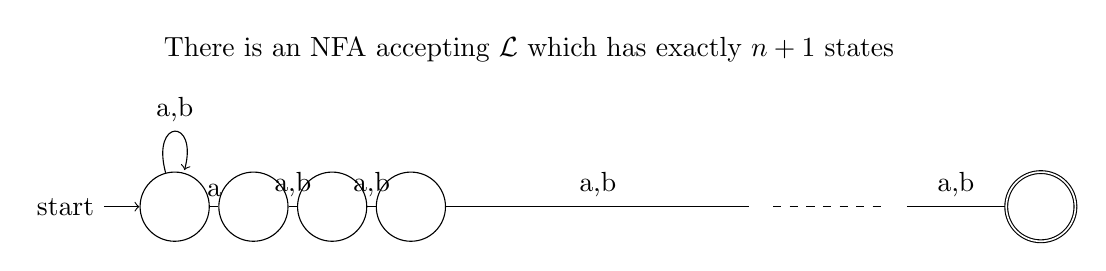
\begin{tikzpicture}
        \node[align=center] at (4.5, 2) {There is an NFA accepting {$\mathcal{L}$} which has exactly $n+1$ states};
        \node[state, initial] (0) {};
        \node[state, right of=0] (1) {};
        \node[state, right of=1] (2) {};
        \node[state, right of=2] (3) {};
        \node[state, accepting] at (11, 0) (4) {};
        \draw (0) edge[loop above] node{a,b} (0)
        (0) edge[above] node{a} (1)
        (1) edge[above] node{a,b} (2)
        (2) edge[above] node{a,b} (3)
        ;
        \draw (7.3,0) coordinate(p1)[label={[label distance=0.9cm]0:$$}]; 
        \draw (9.3,0) coordinate(p2)[label={[label distance=0.9cm]0:$$}]; 
        \draw (7.6,0) coordinate(p3)[label={[label distance=0.9cm]0:$$}]; 
        \draw (9.0,0) coordinate(p4)[label={[label distance=0.9cm]0:$$}]; 
        \draw (3) edge[above] node{a,b} (p1);
        \draw[dashed] (p3) -- (p4);
        \draw (p2) edge[above] node{a,b} (4);
    \end{tikzpicture}
\end{document}
